\documentclass[../../../../../../dd.tex]{subfiles}

\begin{document}

	\subsection{Data Tier}
	This part represents the model of the system ( using a MVC architecture ), so the classes used in this section are the representation of the information that must be stored to use the system.
	\subsubsection{Database} The database is the data structure, so aren't specified the classes used by it, all the information stored are managed by the Database Manager.
	\subsubsection{Database Manager}
	The main classes used to represent the stored data of the application are:
	\begin{itemize}
	\item{Registered User}: this class contains the information about the registered user.
	\item{Taxi Driver}: this class extends the Registered User class and represents the information about the taxi drivers 
	\item{Customer}: this class extends the Registered User class and represents the information about the customers
	\item{Zone}: this class represents the information about the zones. In this class is also stored the queue of the taxi drivers that are available in this specific zone.
	\item{Ride}: this class contains the general information that Ride and Request share. This abstract class follows the pattern State to represent the state of a ride. All Rides start in the state NOT\textunderscore HANDLED, then they can pass to the  state HANDLED, then from this state they can pass to the state NOT\textunderscore HANDLED.
	\item{Request}: this class extends the Ride class and represents the information of the requests for a ride.
	\item{Reservation}: this class extends the Ride class by adding information about the starting and the ending position, and the time of the meeting. Adding this information can be represented the reservation in the system.
	
	\end{itemize}
	
	
	\begin{figure}[H]
				\centering
				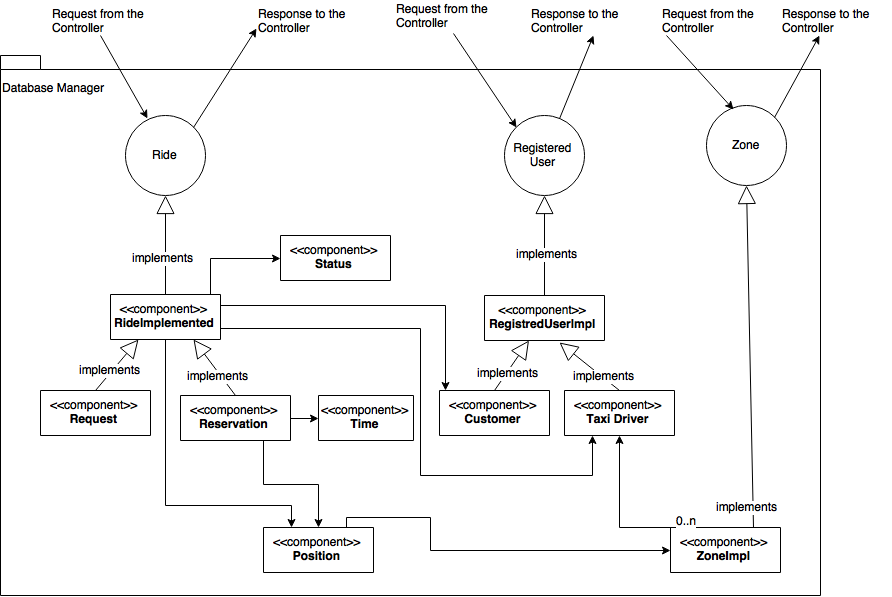
\includegraphics[width=\textwidth, scale=0.5]{../images/DataTier.png}
			\caption{Data Manager Structure}\label{fig:DBMS}
		\end{figure}
	
	
	 
\end{document}